\def\usewhat{pdflatex}

% book作为文档类
% 插入空白页可以设置openright
\documentclass[12pt,openany,oneside]{book}

% 定义本文所使用宏包
%%%%%%%%%% Package %%%%%%%%%%%%

\usepackage{float}
\usepackage{wrapfig}

% 支持插图处理
\usepackage{graphicx}
\usepackage[a4paper,text={146.4true mm,239.2 true mm},top= 26.2true mm,left=31.8 true mm,head=6true mm,headsep=6.5true mm,foot=16.5true mm]{geometry}

% 支持版面尺寸设置
% 支持国际标准单位
\usepackage[squaren]{SIunits}               

\usepackage{titlesec}                       % 控制标题的宏包
\usepackage{titletoc}                       % 控制目录的宏包
\usepackage{fancyhdr}                       % fancyhdr宏包 支持页眉和页脚的相关定义
\usepackage[UTF8]{ctex}                     % 支持中文显示
\usepackage{CJKpunct}                       % 精细调整中文的标点符号
\usepackage{color}                          % 支持彩色
\usepackage{amsmath}                        % AMSLaTeX宏包 用来排出更加漂亮的公式
\usepackage{amssymb}                        % 数学符号生成命令
\usepackage[below]{placeins}    %允许上一个section的浮动图形出现在下一个section的开始部分,还提供\FloatBarrier命令,使所有未处理的浮动图形立即被处理
\usepackage{multirow}                       % 使用Multirow宏包,使得表格可以合并多个row格
\usepackage{booktabs}                       % 表格,横的粗线;\specialrule{1pt}{0pt}{0pt}
\usepackage{longtable}                      % 支持跨页的表格。
\usepackage{tabularx}                       % 自动设置表格的列宽
\usepackage{subfigure}                      % 支持子图 %centerlast 设置最后一行是否居中
\usepackage[subfigure]{ccaption}            % 支持子图的中文标题
\usepackage[sort&compress,numbers]{natbib}  % 支持引用缩写的宏包
\usepackage{enumitem}                       % 使用enumitem宏包,改变列表项的格式
\usepackage{calc}                           % 长度可以用+ - * / 进行计算
\usepackage{txfonts}                        % 字体宏包
\usepackage{bm}                             % 处理数学公式中的黑斜体的宏包
\usepackage[amsmath,thmmarks,hyperref]{ntheorem}  % 定理类环境宏包,其中 amsmath 选项用来兼容 AMS LaTeX 的宏包
\usepackage{CJKnumb}                        % 提供将阿拉伯数字转换成中文数字的命令
\usepackage{indentfirst}                    % 首行缩进宏包
\usepackage{CJKutf8}                        % 用在UTF8编码环境下,它可以自动调用CJK,同时针对UTF8编码作了设置
\usepackage{geometry}
\geometry{left=3.0cm,right=2.0cm,top=2.5cm,bottom=2.5cm}
%\usepackage{hypbmsec}                      % 用来控制书签中标题显示内容
\newcommand{\tabincell}[2]{\begin{tabular}{@{}#1@{}}#2\end{tabular}}
\usepackage{xcolor}
%支持代码环境
\usepackage{listings}
\lstset{numbers=left,
language=[ANSI]{C},
numberstyle=\tiny,
extendedchars=false,
showstringspaces=false,
breakatwhitespace=false,
breaklines=true,
captionpos=b,
%keywordstyle=\color{blue!70},
commentstyle=\color{red!50!green!50!blue!50},
%frame=shadowbox,     %阴影边框
%frame=single,          %单线边框
%不加则无边框
rulesepcolor=\color{red!20!green!20!blue!20}
}
%支持算法环境
\usepackage[boxed,ruled,lined]{algorithm2e}
\usepackage{algorithmic}

\usepackage{times}%times字体
\usepackage{lipsum}


\usepackage{array}
\newcommand{\PreserveBackslash}[1]{\let\temp=\\#1\let\\=\temp}
\newcolumntype{C}[1]{>{\PreserveBackslash\centering}p{#1}}
\newcolumntype{R}[1]{>{\PreserveBackslash\raggedleft}p{#1}}
\newcolumntype{L}[1]{>{\PreserveBackslash\raggedright}p{#1}}

% 生成有书签的 pdf 及其生成方式。通常可以在 tjumain.tex 文件的第一行选择 pdflatex 或者是 dvipdfmx 编译手段。如果选择前者,则使用 pdflatex + pdflatex 编译; 如果选择后者,在编译的时候选择 latex + bibtex + latex + latex 编译。出现混淆的时候,系统会报错。
% 如果您的pdf制作中文书签有乱码使用如下命令,就可以解决了
\def\atemp{dvipdfmx}\ifx\atemp\usewhat
\usepackage[dvipdfmx,unicode,               % dvipdfmx 编译, 加入了中文复制,粘贴支持引擎。
            pdfstartview=FitH,
            bookmarksnumbered=true,
            bookmarksopen=true,
            colorlinks=false,
            pdfborder={0 0 1},
            citecolor=blue,
            linkcolor=red,
            anchorcolor=green,
            urlcolor=blue,
            breaklinks=true
            ]{hyperref}
\fi

\def\atemp{pdflatex}\ifx\atemp\usewhat
\usepackage{cmap}                           % pdflatex 编译时,可以生成可复制、粘贴的中文 PDF 文档, 缺点是在Windows上显示时效果不大好,字体发虚
\usepackage[pdftex,unicode,
            %CJKbookmarks=true,
            bookmarksnumbered=true,
            bookmarksopen=true,                       
            hidelinks
%            colorlinks=true,       % original false
%            pdfborder={0 0 1},
%            citecolor=black,       % original blue
%            linkcolor=black,       % original red
%            anchorcolor=black,           % original green
%            urlcolor=blue,
%            breaklinks=false       % original true
            ]{hyperref}
\fi


% 新增for url
\usepackage{url}

%全局设置表格/图片/公式的编号,而不是1.2之类的
\usepackage{remreset}
\makeatletter
\@removefromreset{table}{chapter}
\@removefromreset{figure}{chapter}
\@removefromreset{equation}{chapter}
\makeatother
\renewcommand{\thetable}{\arabic{table}}
\renewcommand{\thefigure}{\arabic{figure}}
\renewcommand{\theequation}{\arabic{equation}}

\newcommand{\chref}[1]{第~\ref{#1}~章}
\newcommand{\secref}[1]{第~\ref{#1}~节}
\newcommand{\figref}[1]{图~\ref{#1}~}
\newcommand{\tabref}[1]{表~\ref{#1}~}
\newcommand{\equaref}[1]{公式~\eqref{#1}~}


\usepackage{amsmath}
\usepackage{url}
\usepackage{float}
\usepackage{graphicx}
\usepackage{subfigure}
\usepackage{booktabs} 
\usepackage{array}
\usepackage{listings}

\newcommand{\chref}[1]{第~\ref{#1}~章}
\newcommand{\secref}[1]{第~\ref{#1}~节}
\newcommand{\figref}[1]{图~\ref{#1}~}
\newcommand{\tabref}[1]{表~\ref{#1}~}
\newcommand{\equaref}[1]{公式~\eqref{#1}~}

% 定义所有的.eps/.pdf图片文件在figure子目录下
\graphicspath{{figure/}}

\begin{document}

% 开始中文字体使用
\begin{CJK*}{UTF8}{song}

% 完成对论文各个部分格式的设置
%%%%%%%%%%%%%%%%% 图片浮动设置 %%%%%%%%%%%%%%%%%
\setcounter{topnumber}{2}
\setcounter{bottomnumber}{2}
\setcounter{totalnumber}{4}
\renewcommand{\topfraction}{0.85}
\renewcommand{\bottomfraction}{0.85}
\renewcommand{\textfraction}{0.15}
\renewcommand{\floatpagefraction}{0.8}
\renewcommand{\textfraction}{0.1}
\setlength{\floatsep}{5pt plus 2pt minus 2pt}
\setlength{\textfloatsep}{5pt plus 2pt minus 2pt}
\setlength{\intextsep}{5pt plus 2pt minus 2pt}

%%%%%%%%%%%%%%%%% Fonts Definition and Basics %%%%%%%%%%%%%%%%%
\newcommand{\song}{\CJKfamily{song}}    % 宋体
\newcommand{\fs}{\CJKfamily{fs}}        % 仿宋体
\newcommand{\kai}{\CJKfamily{kai}}      % 楷体
\newcommand{\hei}{\CJKfamily{hei}}      % 黑体
\newcommand{\li}{\CJKfamily{li}}        % 隶书
\newcommand{\chuhao}{\fontsize{28pt}{28pt}\selectfont}       % 初号, 单倍行距
\newcommand{\yihao}{\fontsize{26pt}{26pt}\selectfont}       % 一号, 单倍行距
\newcommand{\xiaoyi}{\fontsize{24pt}{24pt}\selectfont}      % 小一, 单倍行距
\newcommand{\erhao}{\fontsize{22pt}{1.25\baselineskip}\selectfont}       % 二号, 1.25倍行距
\newcommand{\xiaoer}{\fontsize{18pt}{18pt}\selectfont}      % 小二, 单倍行距
\newcommand{\sanhao}{\fontsize{16pt}{16pt}\selectfont}      % 三号, 单倍行距
\newcommand{\xiaosan}{\fontsize{15pt}{15pt}\selectfont}     % 小三, 单倍行距
\newcommand{\sihao}{\fontsize{14pt}{14pt}\selectfont}       % 四号, 单倍行距
\newcommand{\xiaosi}{\fontsize{12pt}{12pt}\selectfont}      % 小四, 单倍行距
\newcommand{\wuhao}{\fontsize{10.5pt}{10.5pt}\selectfont}   % 五号, 单倍行距
\newcommand{\xiaowu}{\fontsize{9pt}{9pt}\selectfont}        % 小五, 单倍行距

% 重新定义了波浪符~的意义
\CJKtilde

% 定义章的pre-post名称
\newcommand\prechaptername{第}
\newcommand\postchaptername{章}

% 调整中文字符的表示,行内占一个字符宽度,行尾占半个字符宽度
% 行末半角?
\punctstyle{hangmobanjiao}             

% 调整罗列环境的布局
\setitemize{leftmargin=3em,itemsep=0em,partopsep=0em,parsep=0em,topsep=-0em}
\setenumerate{leftmargin=3em,itemsep=0em,partopsep=0em,parsep=0em,topsep=0em,label={(\arabic*)}}

% 避免宏包 hyperref 和 arydshln 不兼容带来的目录链接失效的问题。
\def\temp{\relax}
\let\temp\addcontentsline
\gdef\addcontentsline{\phantomsection\temp}

% 自定义项目列表标签及格式 \begin{publist} 列表项 \end{publist}
\newcounter{pubctr} %自定义新计数器
\newenvironment{publist}{%%%%%定义新环境
\begin{list}{[\arabic{pubctr}]} %%标签格式
    {
     \usecounter{pubctr}
     \setlength{\leftmargin}{2.5em}   % 左边界 \leftmargin =\itemindent + \labelwidth + \labelsep
     \setlength{\itemindent}{0em}     % 标号缩进量
     \setlength{\labelsep}{1em}       % 标号和列表项之间的距离,默认0.5em
     \setlength{\rightmargin}{0em}    % 右边界
     \setlength{\topsep}{0ex}         % 列表到上下文的垂直距离
     \setlength{\parsep}{0ex}         % 段落间距
     \setlength{\itemsep}{0ex}        % 标签间距
     \setlength{\listparindent}{0pt}  % 段落缩进量
    }}
{\end{list}}

\makeatletter
	\renewcommand\normalsize{
		\@setfontsize\normalsize{12pt}{12pt} % 小四对应 12 pt
		\setlength\abovedisplayskip{4pt}
		\setlength\abovedisplayshortskip{4pt}
		\setlength\belowdisplayskip{\abovedisplayskip}
		\setlength\belowdisplayshortskip{\abovedisplayshortskip}
		\let\@listi\@listI}
	
	% 不同的行距设置
	% TJU原始值1.63
	% 设为1.8则一页31行,1.95则一页29行(目前采用值)(约1.5倍行距)
	\def\defaultfont{\renewcommand{\baselinestretch}{1.95}\normalsize\selectfont} % 设置行距,正文一页29行
	
	% 控制字间距,使每行 34 个汉字
	\renewcommand{\CJKglue}{\hskip -0.1 pt plus 0.08\baselineskip} 
\makeatother

%%%%%%%%%%%%% Contents 目录 %%%%%%%%%%%%%%%%%

\renewcommand{\contentsname}{目录}

% 控制目录深度,改为1
\setcounter{tocdepth}{1}

\titlecontents{chapter}[2em]{\vspace{.0\baselineskip}\sihao\song}	% 可以重调skip
	{\prechaptername~\CJKnumber{\thecontentslabel}~\postchaptername\quad}{}
	{\!\titlerule*[5pt]{$\cdot$}\!\!\!\!\sihao\contentspage}	% 调整点的距离
\titlecontents{section}[3em]{\vspace{-0.1\baselineskip}\xiaosi\song}
	{\thecontentslabel\quad}{}
	{\!\titlerule*[5pt]{$\cdot$}\!\!\!\!\xiaosi\contentspage}
\titlecontents{subsection}[4em]{\vspace{-0.2\baselineskip}\wuhao\song}
	{\thecontentslabel\quad}{}
	{\!\titlerule*[5pt]{$\cdot$}\!\!\!\!\wuhao\contentspage}
             
%%%%%%%%%% Chapter and Section 章节 %%%%%%%%%%%%%

\setcounter{secnumdepth}{4}
\setlength{\parindent}{2em}

% 如果使用第“一”章
\renewcommand{\chaptername}{\prechaptername\CJKnumber{\thechapter}\postchaptername}
% 使用第“1”章
%\renewcommand{\chaptername}{\thechapter}

% 此处修改的chapter title会被主文件定义覆盖
% chapter标题格式:小二,黑体,居中
\titleformat{\chapter}{\centering\xiaoer\hei}{\chaptername}{2em}{}
\titlespacing{\chapter}{0pt}{0.1\baselineskip}{0.8\baselineskip}

% section标题格式:四号,黑体,左对齐
\titleformat{\section}{\sihao\hei}{\thesection}{1em}{}
\titlespacing{\section}{0pt}{0.15\baselineskip}{0.25\baselineskip}

% subsection标题格式:小四,黑体,左对齐
\titleformat{\subsection}{\xiaosi\hei}{\thesubsection}{1em}{}
\titlespacing{\subsection}{0pt}{0.1\baselineskip}{0.3\baselineskip}

% subsubsection标题格式:小四,宋体加粗,左对齐
\titleformat{\subsubsection}{\xiaosi\song\bfseries}{\thesubsubsection}{1em}{}
\titlespacing{\subsubsection}{0pt}{0.05\baselineskip}{0.1\baselineskip}

%%%%%%%%%% Table, Figure and Equation 图/表/公式 %%%%%%%%%%%%%%%%%

\renewcommand{\tablename}{表}
\renewcommand{\figurename}{图}

% 使图编号为 7-1 的格式
%\renewcommand{\thefigure}{\arabic{chapter}-\arabic{figure}}
%按顺序编号
%\renewcommand{\thefigure}{\arabic{figure}}
% 使子图编号为 a) 的格式
%\renewcommand{\thesubfigure}{\alph{subfigure})}
% 使子图编号为 (a) 的格式
\renewcommand{\thesubfigure}{(\alph{subfigure})}

% 使子表编号为 (a) 的格式
\renewcommand{\thesubtable}{(\alph{subtable})}
% 使表编号为 7-1 的格式
%\renewcommand{\thetable}{\arabic{chapter}-\arabic{table}}
%按顺序编号
\renewcommand{\thetable}{\arabic{table}}
% 使公式编号为 7-1 的格式
%\renewcommand{\theequation}{\arabic{chapter}-\arabic{equation}}

\makeatletter
	% 使子图引用也是7-1a)或7-1(a)的形式
	\renewcommand{\p@subfigure}{\thefigure}
\makeatother

% 定制浮动图形和表格标题样式
\makeatletter
	\long\def\@makecaption#1#2{
	   \vskip\abovecaptionskip
	   \sbox\@tempboxa{\centering\wuhao\song\bfseries{#1\quad #2}}
	   \ifdim \wd\@tempboxa >\hsize
	     \centering\wuhao\song{#1\quad #2} \par	% narrower
	   \else
	     \global \@minipagefalse
	     \hb@xt@\hsize{\hfil\box\@tempboxa\hfil}
	   \fi
	   \vskip\belowcaptionskip}
\makeatother

% 用来控制longtable表头分隔符
\captiondelim{~~~~} 

%%%%%%%%%% Theorem Environment 定理 %%%%%%%%%%%%%%%%%
\theoremstyle{plain}
\theorembodyfont{\song\rmfamily}
\theoremheaderfont{\hei\rmfamily}
\newtheorem{theorem}{定理~}[chapter]
\newtheorem{lemma}{引理~}[chapter]
\newtheorem{axiom}{公理~}[chapter]
\newtheorem{proposition}{命题~}[chapter]
\newtheorem{prop}{性质~}[chapter]
\newtheorem{corollary}{推论~}[chapter]
\newtheorem{conclusion}{结论~}[chapter]
\newtheorem{definition}{定义~}[chapter]
\newtheorem{conjecture}{猜想~}[chapter]
\newtheorem{example}{例~}[chapter]
\newtheorem{remark}{注~}[chapter]
%\newtheorem{algorithm}{算法~}[chapter]
\newenvironment{proof}{\noindent{\hei 证明:}}{\hfill $ \square $ \vskip 4mm}
\theoremsymbol{$\square$}

%%%%%%%%%% Page: number, header and footer 页面设置 %%%%%%%%%%%%%%%%%

%\frontmatter 或 \pagenumbering{roman}
%\mainmatter 或 \pagenumbering{arabic}

\makeatletter
	\renewcommand\frontmatter{\clearpage
		\@mainmatterfalse}
\makeatother

%%%%%%%%%%%% References 参考文献 %%%%%%%%%%%%%%%%%

\renewcommand{\bibname}{参考文献}
% 重定义参考文献样式,来自thu
\makeatletter
\renewenvironment{thebibliography}[1]{
    %\titleformat{\chapter}{\raggedright\sihao\hei}{\chaptername}{2em}{}
    %\titleformat{\chapter}{\centering\sihao\hei}{\chaptername}{2em}{}
    %\titleformat{\chapter}{\centering\xiaoer\hei}{\chaptername}{2em}{}
   \chapter*{\bibname}
   \wuhao
   \list{\@biblabel{\@arabic\c@enumiv}}
        {\renewcommand{\makelabel}[1]{##1\hfill}
         \settowidth\labelwidth{0 cm}
         \setlength{\labelsep}{0pt}
         \setlength{\itemindent}{0pt}
         \setlength{\leftmargin}{\labelwidth+\labelsep}
         \addtolength{\itemsep}{-0.7em}
%         \addtolength{\itemsep}{-1.0em}
         \linespread{1.5}\selectfont	% 调整每个参考文献项内的间距 !!!
         \usecounter{enumiv}
         \let\p@enumiv\@empty
         \renewcommand\theenumiv{\@arabic\c@enumiv}}
    \sloppy\frenchspacing
    \clubpenalty4000
    \@clubpenalty \clubpenalty
    \widowpenalty4000
    \interlinepenalty4000
    \sfcode`\.\@m}
   {\def\@noitemerr
     {\@latex@warning{Empty `thebibliography' environment}}
    \endlist\frenchspacing}
\makeatother

% 缩小参考文献间的垂直间距
\addtolength{\bibsep}{-0.5em}

% 每个条目自第二行起缩进的距离
\setlength{\bibhang}{2em}

% 参考文献引用作为上标出现
\makeatletter
	\def\@cite#1#2{\textsuperscript{[{#1\if@tempswa , #2\fi}]}}
\makeatother

% 引用格式
\bibpunct{[}{]}{,}{s}{}{,}

%%%%%%%%%%%% Cover 封面、摘要、版权、致谢格式定义 %%%%%%%%%%%%%%%%%
 
\makeatletter % 一直到结尾

\def\ctitle#1{\def\@ctitle{#1}}\def\@ctitle{}
\def\etitle#1{\def\@etitle{#1}}\def\@etitle{}
\def\subtitle#1{\def\@subtitle{#1}}\def\@subtitle{}
\def\esubject#1{\def\@esubject{#1}}\def\@esubject{}
\def\cauthor#1{\def\@cauthor{#1}}\def\@cauthor{}
\def\eauthor#1{\def\@eauthor{#1}}\def\@eauthor{}
\def\csupervisor#1{\def\@csupervisor{#1}}\def\@csupervisor{}
\def\esupervisor#1{\def\@esupervisor{#1}}\def\@esupervisor{}
\def\cdate#1{\def\@cdate{#1}}\def\@cdate{}
\long\def\cabstract#1{\long\def\@cabstract{#1}}\long\def\@cabstract{}
\long\def\eabstract#1{\long\def\@eabstract{#1}}\long\def\@eabstract{}
\def\ckeywords#1{\def\@ckeywords{#1}}\def\@ckeywords{}
\def\ekeywords#1{\def\@ekeywords{#1}}\def\@ekeywords{}
\def\cheading#1{\def\@cheading{#1}}\def\@cheading{}

\pagestyle{fancy}
  \fancyhf{}
  \fancyhead[C]{\song\wuhao \@cheading}  % 页眉
%  \lhead{\song\wuhao \@cheading}  % 左页眉
%  \rhead{\prechaptername\CJKnumber{\thechapter}\postchaptername}    % 右页眉
%  \rhead{\prechaptername~\thechapter~\postchaptername}    % 右页眉
  \fancyfoot[C]{\song\xiaowu ~\thepage~}
\newlength{\@title@width}

% 定义封面
\def\makecover{
   \phantomsection
    \pdfbookmark[-1]{\@ctitle}{ctitle}

\begin{titlepage}
%\vspace*{31.5pt}
\begin{center}
  %\vspace*{21pt}
\setlength{\parindent}{2em}
  \begin{figure}[!h]
  \flushleft
  \hspace*{4pt}
  
\includegraphics[width=3.18cm]{icon.png}
  \end{figure}

  \vspace*{21pt}
  \begin{figure}[!h]
  \centering
  
\includegraphics[width=11.34cm]{name.png}
  \end{figure}
  \vspace*{42pt}

  \song\erhao{\textbf{第三十一届“冯如杯”学生学术科技作品竞赛项目论文}}

  \vspace*{110pt}
  \song\erhao{\@ctitle}

  \begin{flushright}
  \sanhao{\textrm{\@subtitle}}
  \end{flushright}

 
   \vspace*{42pt}
    \setlength{\@title@width}{5cm}

 % \vspace*{60pt}

 %  \vspace*{21pt}
\vfill
\sanhao{\textbf{\@cdate}}
\end{center}
\end{titlepage}


%%%%%%%%%%%%%%%%%%% Abstract and Keywords 摘要和关键词 %%%%%%%%%%%%%%%%%%%%%%%

%中文摘要格式
\clearpage
\markboth{摘要}{摘要}
\pdfbookmark[0]{摘要}{cabstract}

% 摘要不加到目录中
%\addcontentsline{toc}{chapter}{摘要}

% 开始罗马数字编号
\setcounter{page}{1}
\pagenumbering{roman}
\thispagestyle{plain}


% 中文摘要:小二,黑体加粗,居中
\begin{center}
% \xiaosan\hei\bfseries 摘要
\xiaosan\hei 摘要
\end{center}

%\vspace{\baselineskip} % 新增摘要后空行

% 插入中文摘要
\song\defaultfont
\@cabstract
% \vspace{\baselineskip}

%\hangafter=1\hangindent=52.3pt\noindent
\hangafter=1\hangindent=52.3pt
{\hei\xiaosi 关键词:} \@ckeywords
%\thispagestyle{empty}

% 英文摘要格式
\clearpage
 \markboth{Abstract}{Abstract}
 \pdfbookmark[0]{Abstract}{eabstract}

 % 摘要不加到目录中
 %\addcontentsline{toc}{chapter}{ABSTRACT}

 \thispagestyle{plain}

% ABSTRACT三号居中
 \begin{center}
 % \sanhao{\bf{Abstract}}
 \sanhao{Abstract}
 \end{center}
% \vspace{\baselineskip}

% 插入英文摘要
\@eabstract
% \vspace{\baselineskip}

% \hangafter=1\hangindent=60pt\noindent
\hangafter=1\hangindent=60pt
{\textbf{Keywords:}} \@ekeywords
\thispagestyle{plain}

}
\makeatother
     

% ——————————————————————————————————————————————
% 以下是论文导言部分,包括论文的封面,中英文摘要和中文目录

\frontmatter
\fancypagestyle{plain}{
\fancyhf{}
\renewcommand{\headrulewidth}{0 pt}

\fancyfoot[C]{\xiaowu\thepage}
}

%%%%%%%%%%   封面   %%%%%%%%%%

% !Mode:: "TeX:UTF-8"
%!TEX root = ../main.tex
\cheading{北京航空航天大学第三十一届“冯如杯”学生学术科技作品竞赛参赛作品}      % 设置正文的页眉

\ctitle{AirBand手环}    % 封面用论文标题,自己可手动断行

%\etitle{Thesis English Title}    %论文英文标题

\subtitle{——基于NFC技术的智能社交手环}   % 副标题


% 自动数字日期
\cdate{\the\year~年~\the\month~月}

\cabstract{

近年来,智能可穿戴设备领域正在迅速升温。
PS:latex里貌似没有华文中宋和华文新魏字体。建议使用Acrobat神器将封面替换。

}

\ckeywords{冯如杯;LAtex模板;关键词}

\eabstract{
\lipsum[1-2]
}

\ekeywords{Fengrubei; thesis; template; use commas or colons to separate}

\makecover

\clearpage


%%%%%%%%%%   摘要   %%%%%%%%%%

\cabstract{

近年来,智能可穿戴设备领域正在迅速升温。
PS:latex里貌似没有华文中宋和华文新魏字体。建议使用Acrobat神器将封面替换。

}

\ckeywords{冯如杯;LAtex模板;关键词}

\eabstract{
\lipsum[1-2]
}

\ekeywords{Fengrubei; thesis; template; use commas or colons to separate}

\makecover

\clearpage

%%%%%%%%%%   目录   %%%%%%%%%%
\defaultfont
%\clearpage{\pagestyle{empty}\cleardoublepage}
\clearpage
%\pagestyle{empty}
%\setcounter{page}{1}                                 % 单独从 1 开始编页码
%\pagenumbering{arabic}
\titleformat{\chapter}{\centering\sanhao\hei}{\chaptername}{2em}{} % 设置目录两字的格式

\tableofcontents                                     % 中文目录


\thispagestyle{plain}

% ——————————————————————————————————————————————
% 以下是论文正文,内容在body子文件夹下

\mainmatter\defaultfont\sloppy\raggedbottom
\makeatletter
	\fancypagestyle{plain}{                              % 设置开章页眉页脚风格
		\fancyhf{}
		\fancyhead[C]{\song\wuhao \@cheading}            % 首页页眉格式
		\fancyfoot[C]{\song\xiaowu ~\thepage~}           % 首页页脚格式
		\renewcommand{\headrulewidth}{0.5pt}
		\renewcommand{\footrulewidth}{0pt}}
\makeatother


% 单独从 1 开始编页码
\setcounter{page}{1}
% chapter标题格式:三号,黑体,左对齐
\titleformat{\chapter}{\centering\sanhao\hei}{\chaptername}{2em}{}

%%%%%%%%%%   正文   %%%%%%%%%%

\chapter{问题背景}
\section{项目背景}
\subsection{背景一}
随着谷歌、三星和苹果等科技巨头相继投入巨资开发可穿戴设备产品,该领域市场在年逐渐升温\cite{wu2013online}。


\subsection{背景二}
随着谷歌、三星和苹果等科技巨头相继投入巨资开发可穿戴设备产品,该领域市场在年逐渐升温。 

\subsection{项目制作的目的与意义}
我们制作了一款智能手环。

\subsection{项目创新点}
AirBand智能手环采用NFC芯片与低功耗蓝牙芯片结合。

\begin{equation}
    1+2
    \label{alg:abc}
\end{equation}

看这个\equaref{alg:abc}
\chapter{嵌入式智能硬件设计}
\section{总体设计}
该智能设备的硬件设计如下。


\section{硬件模块}

\section{NFC模块}
如图\ref{pn532}所示是PN532芯片。

\begin{figure}[!h]
 \centering
 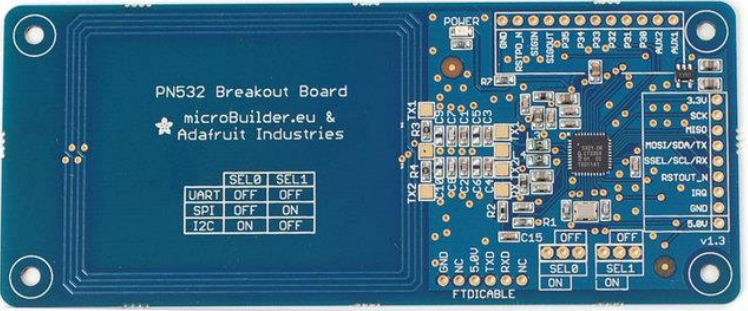
\includegraphics[width=8cm]{pn532.png}
 \caption{PN532芯片}
 \label{pn532}
\end{figure}



 % \begin{figure}[h]
 % \begin{minipage}{0.48\linewidth}
 %   \centerline{\includegraphics[width=8cm]{2.png}}
 %   \centerline{\tiny{(a) 子图1}}
 % \end{minipage}
 % \hfill
 % \begin{minipage}{0.48\linewidth}
 %   \centerline{\includegraphics[width=8cm]{1.jpg}}
 %   \centerline{\tiny{(b) 子图2}}
 % \end{minipage}
 % \vfill
 % \caption{子图12对比}
 % \end{figure}

\section{BLE通信模块}

BLE通信模块主要包括蓝牙芯片以及蓝牙天线和其外围电路,其电路原理如下。
\chapter{说明}


\section{使用方法}
\label{sec:usage}

本模板只包括内容方面的设计预定义,编译自行解决。作者使用的是Windows环境下MikTex+TeXstudio的组合。

\section{使用建议}
\label{sec:tips}

\subsection{普适问题}
\label{subsec:common}

普遍适用的论文排版问题:

\begin{enumerate}
\item 图片标题在下,表格在上;一定要有标题,不能只是图1-1;与文字内容的间隔自行把握。
\item 参考文献建议使用.bib文件;也有使用Google Scholar的引用的,但有指出当中的“//”不符合规范。
\item 部分评审反馈,目录不包含摘要及目录本身,请根据情况自行斟酌。
\item 打印时需要右边翻页的问题(每章开始在右边页),可以在生成pdf后通过插入空白页解决(这样插入不会改变页码);或者尝试设置openright(未测试,有待探讨)。
\end{enumerate}

\subsection{细节问题}
\label{subsec:specs}

一些细节的问题建议:
\begin{itemize}
\item 每个章节都有label,key使用ch:intro形式,以下使用sec:background等。图片key可以参考fig:scenes,表格参考tab:exp。
\item 图片、表格尽量在页的顶部,即float优先选择t。
\item 另外,为了打印时彩打方便,可以把需要彩打的图片尽量排版在一页,不过比较难调。
\item 虽然每个body的tex文件中包含了!Mode:: ``TeX:UTF-8"在文件开头,但仍有必要在IDE中将新建的tex文件设为UTF-8编码,否则可能无法正常显示中文。
\end{itemize}

\subsection{其他说明}
\label{sec:setting}

参考文献目前采用上标表示。使用cite命令。

目前页眉设置:每章第一页页眉只有中间的“中山大学硕士毕业论文”,后续页左边显示“中山大学硕士毕业论文”,右边显示“第n章”。

目前页脚设置:仅包含页码,居中,无横线。

参考文献和附录计算页数,包含在目录,页眉设置同每章第一页。正文前的部分无页眉。

\section{例子}
\label{sec:examples}


表例子。推荐使用这种三行表。缺省值使用三个“-”产生长横线“---”。

\begin{table}[!t]
\caption{示例表}
\label{tab:eg}
\vspace{0.5em}
\centering
\wuhao
  \begin{tabular}{ccccc}
  \toprule[1.5pt]
  表头 & 栏1 & 栏2 & 栏3 & 栏4 \\
  \midrule[1pt]
  内容1 & b & --- & $768 \times 576$ & 19 \\
  内容1 & a & 240/7 & $768 \times 576$ & --- \\
  \bottomrule[1.5pt]
  \end{tabular}
\end{table}

公式例子,与普通Latex数学公式无异。

\begin{equation}
1+1=2
\end{equation}

%%%%%%%%%%  参考文献  %%%%%%%%%%
% \lhead{}
% \rhead{}
% \chead{\song\wuhao 北京航空航天大学第三十一届“冯如杯”学生学术科技作品竞赛参赛作品} % 覆盖设置页眉内容
% \defaultfont
\bibliographystyle{references/FengrubeiStyle}
%\phantomsection
\markboth{参考文献}{参考文献}
\addcontentsline{toc}{chapter}{参考文献}       % 参考文献加入到中文目录


\nocite{*}                                     
% 若将此命令屏蔽掉,则未引用的文献不会出现在文后的参考文献中

%启用此命令:使用.bib文件作为文献来源
\bibliography{references/ref}


% \begin{thebibliography}{99}
% \bibitem{ly}李扬. 新一代智能终端——可穿戴设备[J]. 高科技与产业化,2013,10:82-85.
% \bibitem{tx}Tao Xie and Dengguo Feng. How To Find Weak Input Differences For MD5 Collision Attacks. 30 May 2009.


% \end{thebibliography}

% ——————————————————————————————————————————————
% 以下是论文附录,在appendix子文件下

%%%%%%%%%%   附录   %%%%%%%%%%

\markboth{附录}{附录}
\addcontentsline{toc}{chapter}{附录} % 添加到目录中
%\setcounter{page}{1}       % 如果需要从该页开始从 1 开始编页,则取消该注释

\chapter*{附录}

\section*{主成分分析中的回归方程系数矩阵}

%\begin{enumerate}
	% 盲审时
	%\item The paper title [J/C...]. Publish whereabout, 2014, 21(3): 288-291. (第一作者,导师为第一作者)(与学位论文第n章相关)(盲审时,不要出现名字)
	% 提交时
	%\item Authors. The paper title [J/C...]. Publish whereabout, 2014, 21(3): 288-291. (提交时)
%\end{enumerate}


\begin{table}[h]
\centering
\caption{主成分分析中的回归方程系数矩阵}
\begin{tabular}{llllllllllll}
\hline
\multicolumn{1}{c}{\textbf{基因}} & \multicolumn{1}{c}{\textbf{成分1}} & \multicolumn{1}{c}{\textbf{成分2}} & \multicolumn{1}{c}{\textbf{成分3}} & \multicolumn{1}{c}{\textbf{成分4}} & \multicolumn{1}{c}{\textbf{成分5}} & \multicolumn{1}{c}{\textbf{成分6}} & \multicolumn{1}{c}{\textbf{成分7}} & \multicolumn{1}{c}{\textbf{成分8}} & \multicolumn{1}{c}{\textbf{成分9}} & \multicolumn{1}{c}{\textbf{成分10}} & \multicolumn{1}{c}{\textbf{成分11}} \\ \hline
KRT14|3861                      & .134                             & .033                             & -.025                            & .060                             & -.111                            & -.136                            & .193                             & .303                             & -.039                            & -.043                             & -.007                             \\
KRT13|3860                      & .108                             & .050                             & .000                             & .075                             & .247                             & .162                             & -.188                            & -.241                            & .061                             & .015                              & -.002                             \\
SFTPB|6439                      & -.025                            & .032                             & .204                             & .059                             & .004                             & -.010                            & .000                             & .026                             & -.062                            & .000                              & .071                              \\

IGFBP3|3486                     & -.060                            & .113                             & -.120                            & .036                             & -.029                            & -.006                            & -.012                            & -.130                            & .229                             & .100                              & -.028                            \\ \hline
\end{tabular}
\end{table}



% 仍然有页码
%\thispagestyle{empty}

% \markboth{附\quad 录}{附\quad 录}
% \addcontentsline{toc}{chapter}{附\quad 录} % 添加到目录中

\chapter*{源程序}
\lstset{language=C}
\begin{lstlisting}

#include<stdio.h>
#include <stdlib.h>
int main()
{
	FILE *fp1;
	double shuju[180+1][367+1]={0.0};
	double t=0.0;
	double max[180+1]={0};
	int start[180+1]={0};
	int end[180+1]={0};
	FILE *fp2;
	fp2=fopen("C:\\Users\\Dell-pc\\Desktop\\正方形2222.xls","w");
	fprintf(fp2,"shujuzushu\t max\n");
	int i,j=0;
	if(NULL == (fp1 = fopen("C:\\Users\\Dell-pc\\Desktop\\1.txt", "r")))  
    {  
        printf("error\n");  
        exit(1);  
    }
    for(i=1;i<=180;i++)
	{
	 for(j=1;j<=367;j++)
		{
			fscanf(fp1,"%lf",&shuju[i][j]);
			//printf("%lf\n",shuju[i][j]);
		}
		fscanf(fp1,"\n");
	}
	 fclose(fp1);
	
	
	 for(i=1;i<=180;i++)
	{
	
		 for(j=1;j<=367;j++)
		{
			
			
			if(shuju[i][j]==0.0&&shuju[i][j+1]!=0.0)
			{
				start[i]=j+1;
			  }
			  if(shuju[i][j]!=0.0&&shuju[i][j+1]==0.0)
			{
				end[i]=j;
			  }
		}
	}
	for(i=1;i<=180;i++)
	{
		max[i]=(start[i]+end[i])/2;
		fprintf(fp2,"%d\t   %lf\n",i,max[i]);
	}
 }
\end{lstlisting}

% % 重新设置想要的chapter格式
% \titleformat{\chapter}{\raggedright\sihao\hei}{\chaptername}{2em}{}

\clearpage

% 结束中文字体使用
\end{CJK*}

% 结束全文
\end{document}